\chapter{Approach}
% Describe the performed solution with all possible details. Define necessary parameters, inputs, outputs and context of use, possible problems and when they can be applied. 

% Remember to define necessary concepts before using them, building the text from easiest definitions (not depending on previous definitions) to complex definitions (depending on previous definitions).

% E.g: 
% \begin{itemize}
%	\item Lost Communication: a lost communication occurs when the conditions of the environment are not sufficient or the distance between sender and receiver is to hight to transmit information.
%	\item Wait until rescue: when the robot loses its communication, the pre-designed state machine will stop the motors to keep the actual position. Energy safe mode will be enabled, at the same time that a channel transceiver daemon will send SOS messages every T and wait for reply during T sec. 
%\end{itemize}
In our system there are a multiple robots that must handle various tasks. For example, visiting given rooms. To tackele this problem, a communication efficient task scheduling system is designed. 
This system allicate task according to system resources, including enviroment factors and robot available battery. Once these information is attained, the task scheduling system assign robot a set of task.
\begin{itemize}
	\item \textsl{Robot.} The robot is responssible for executing tasks as well as listen to sensors on its way. It has a rechargeable battery. Robot battery level drops as its moves and rotates.
	\item \textsl{Tasks.} The tasks include two part. The first part is moving to a given position and the second part is either finding a person or recharge itself.
	\item \textsl{Enviroment.} The enviroment is an office area that contains a corridor along the central x axis and 16 rooms located around the corridor. The enviroment model is shown in Figure \ref{fig:gazebo_model}. The enviroment factors, such as room location and occupancy possibility help task allocation.
\end{itemize}

\begin{figure}[htbp]
	\centering
	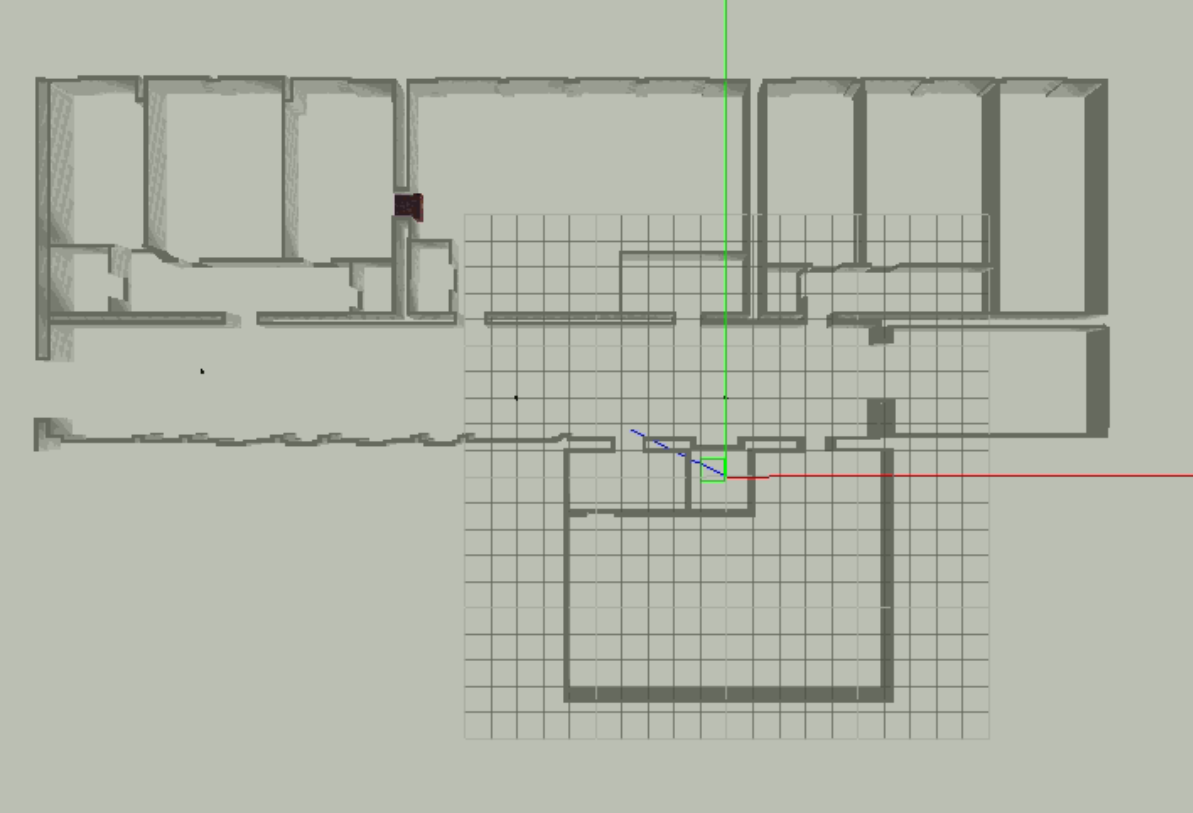
\includegraphics[width = 0.7\textwidth]{content/images/ch3/gazebo_model.png}
	\caption{Gazebo Model}
	\label{fig:gazebo_model}
\end{figure}

\section{Architecture Design}

As shown is Figure \ref{fig:system_architecture}, the architecture of the system consist of several parts: centralized pool, robot controller, navigation stack, charging station and system enviroment. 
\begin{itemize}
	\item \textsl{Centralized Pool.} A centralized pool consist of serveral modules: multi-robot task allocation module, system enviroment state, database, execution and mornitoring. The database contains the room information such as occupancy possible and the tasks. The multirobot task allocation module assign task to robots according to both robot status and system enviroment.
	\item \textsl{Robot Controller.} A robot controller contains serveral modules: execute module and robot action. The execute module receive commands from centralized pool and decide when and which task the robot should perform. During performing a task,a robot can send enviroment information to centralized pool.
	\item \textsl{Navigation stack.} The move\_base node provides a ROS interface for configuring, running, and interacting with the navigation stack on a robot. It make robot move to desired positions using the navigation stack. Its advantages includes optionally performing recovery behaviors when the robot perceives itself as stuck. 
\end{itemize} 

\begin{figure}[htbp]
	\centering
	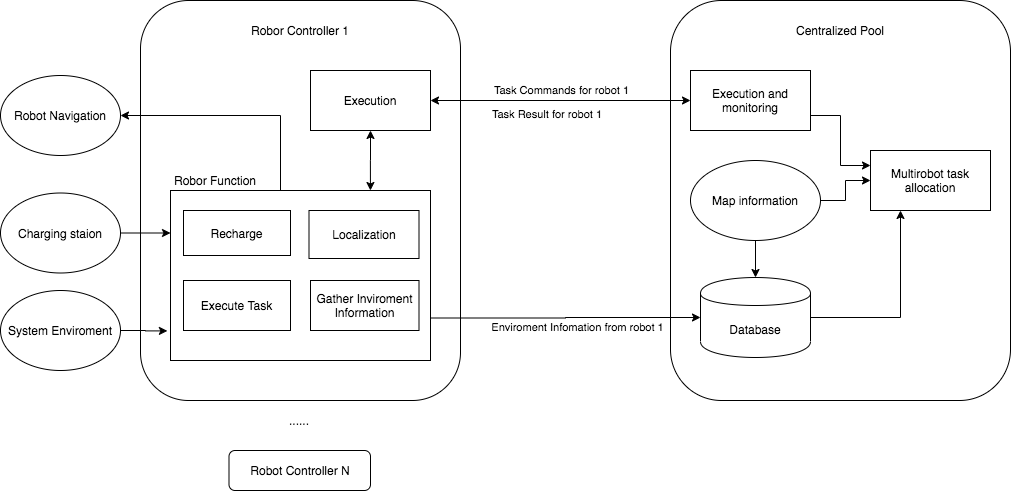
\includegraphics[width = 0.8\textwidth]{content/images/ch3/architecture.drawio.png}
	\caption{System architecture}
	\label{fig:system_architecture}
\end{figure}

\begin{figure}[htbp]
	\centering
	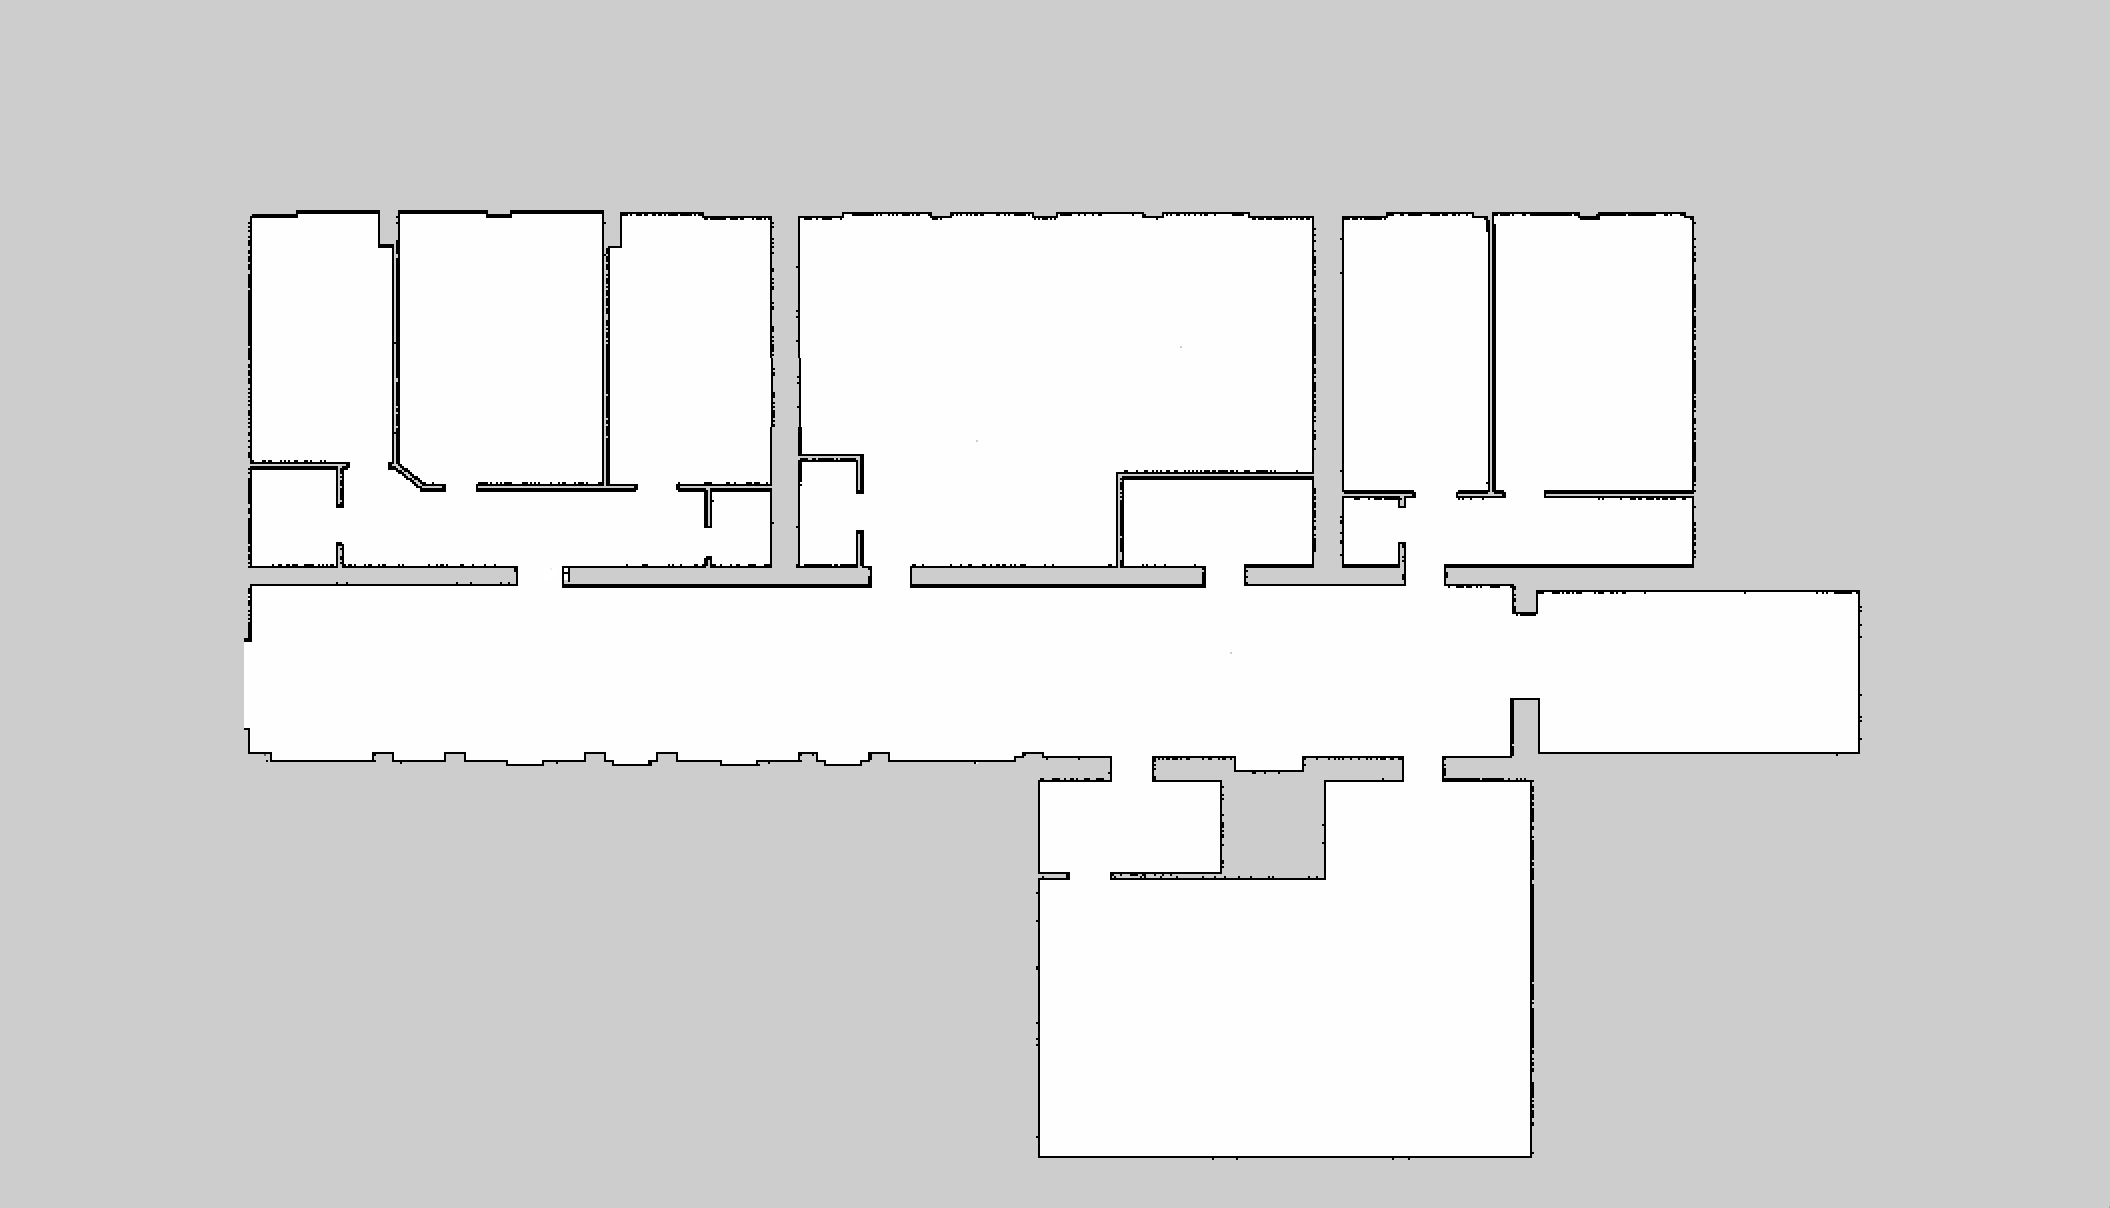
\includegraphics[width = 0.7\textwidth]{content/images/ch3/occupancy_grid.png}
	\caption{Enviroment occupancy grid}
	\label{fig:occupancy_grid}
\end{figure}

\section{System Environment}
The system enviroment is an office area. A 3D Gazebo module shown in \ref{fig:gazebo_model}, and an occupancy grid is shown in \ref{fig:occupancy_grid}. The write area is unoccupied, which is the corridor and rooms. The black line is occuppied area, which is the wall. anything else is gray.
Following are important objects in system enviroment that interact with robot.
\begin{itemize}
	\item \textsl{Room.} As is shown in Fgure \ref{fig:room_division}, the restrict area(the write area in Figure \ref{fig:room_division}) is divided into rectangles. The rectangle is used to let the system clearly distinguish which room robot is in.
	\item \textsl{Door.} In 3D Model there are no original doors. However in order to simulate an enviroment, a few simulated sensors are created. Those coordinate of sensors are the same as corresponding doors positions (D1-D17 in Figure \ref{fig:positions_door_station}).
	Additionally one simulated door sensor is created on the door position. Each simulated door sensors brocasts door status periodically. The broadcast message are received by all robot within its range, including both robots enter the room and robots in corridor passing by the door.
	Figure \ref{fig:positions_door_station} shows the distribution of doors.
	\item \text{Charging Station.} The battery decrease is also considered. Three simulated charging stations are located in the corridor. Figure \ref{fig:positions_door_station} shows the distribution of charging stations. 
	When robot get a charging task, it would move to one of the charging station and wait until fully charged. The details of robot charging is shown in Section \todo{Robot charging}.
	
\end{itemize}

\begin{figure}[htbp]
	\centering
	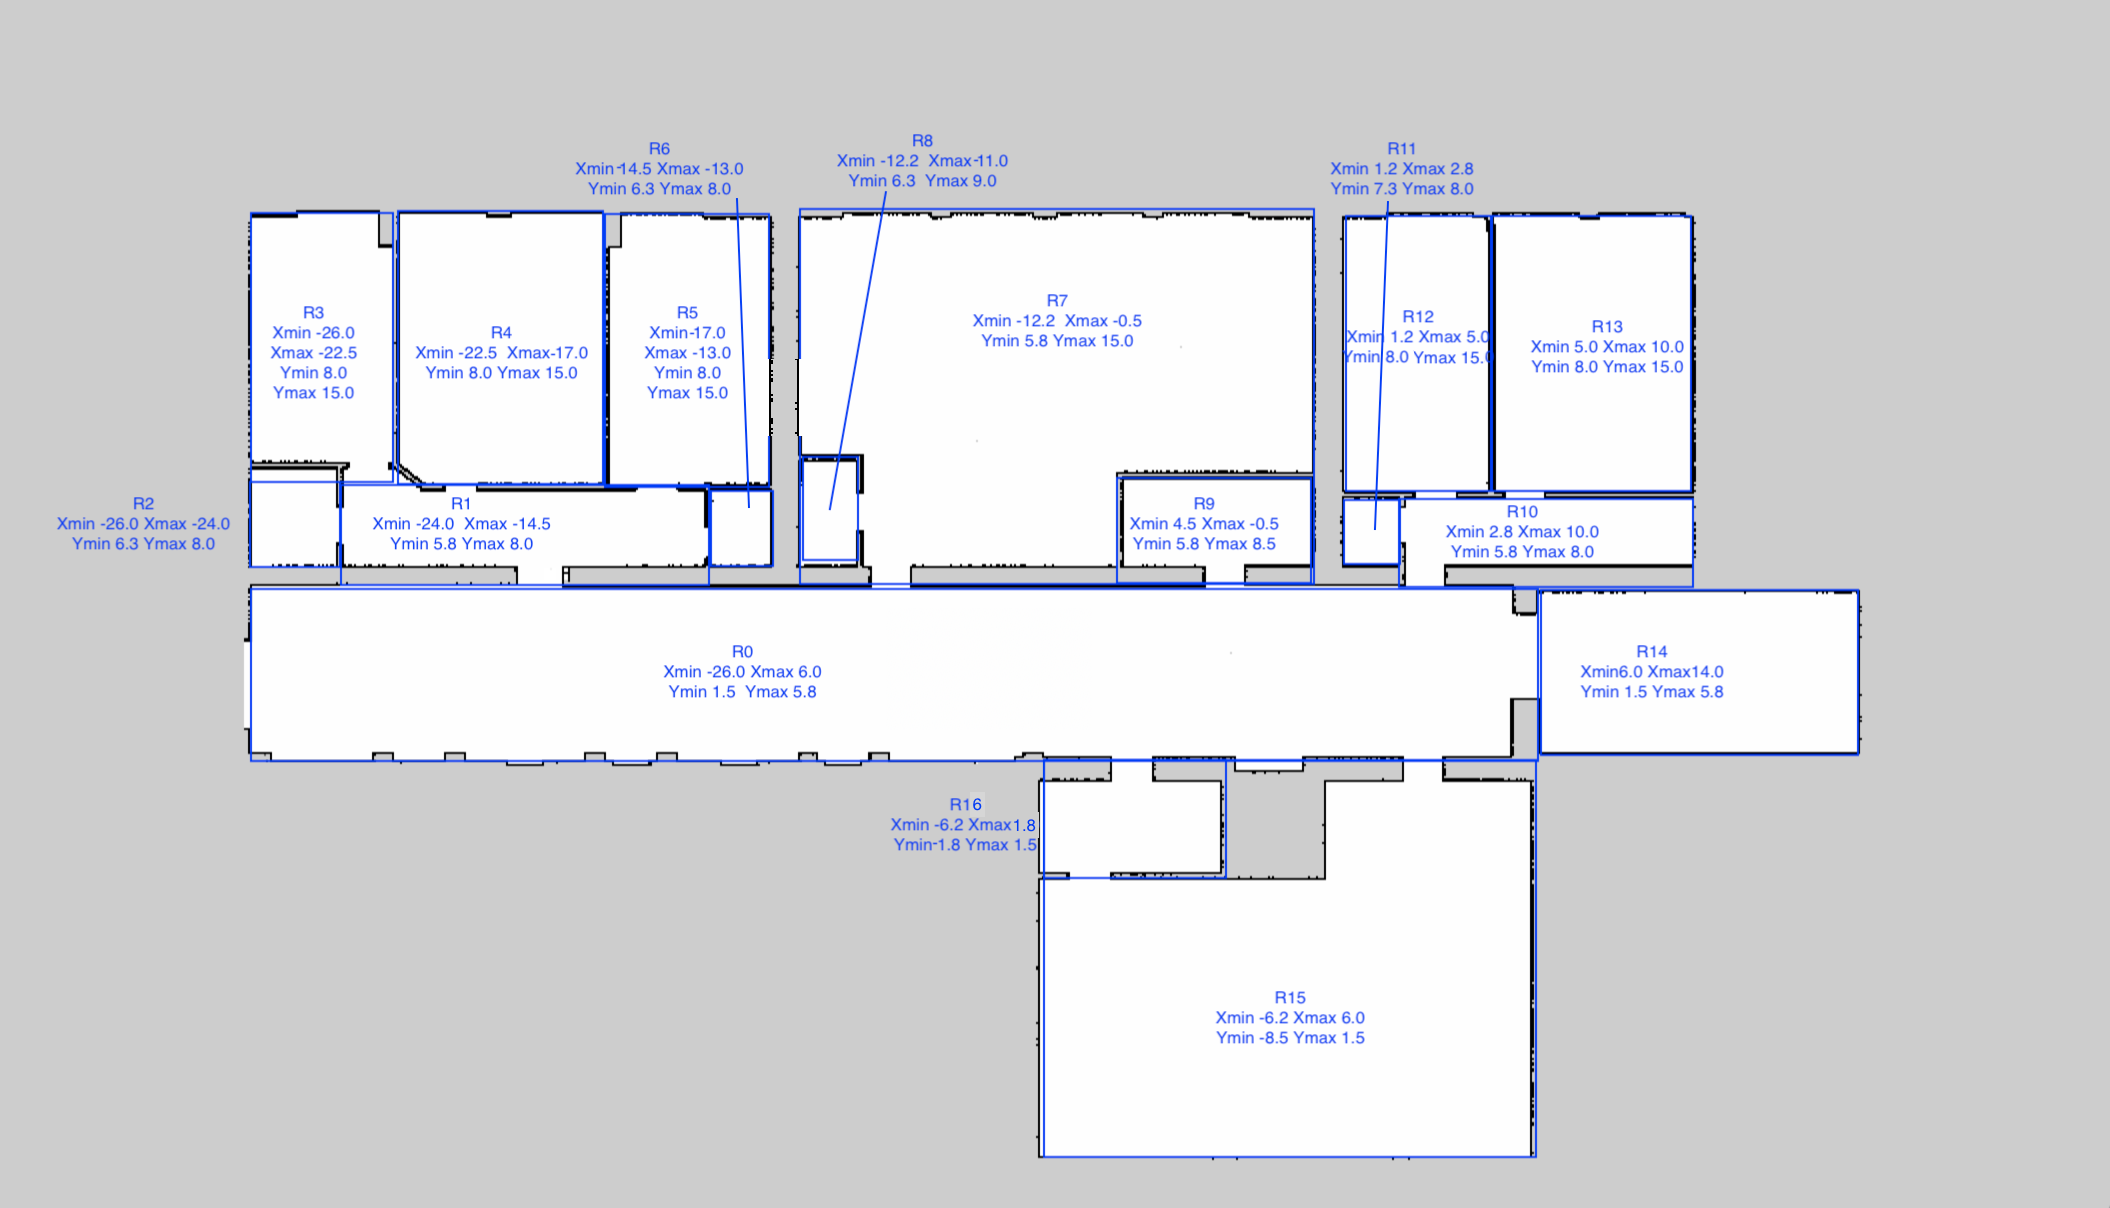
\includegraphics[width = 0.7\textwidth]{content/images/ch3/room_division.png}
	\caption{Room division}
	\label{fig:room_division}
\end{figure}

\begin{figure}[htbp]
	\centering
	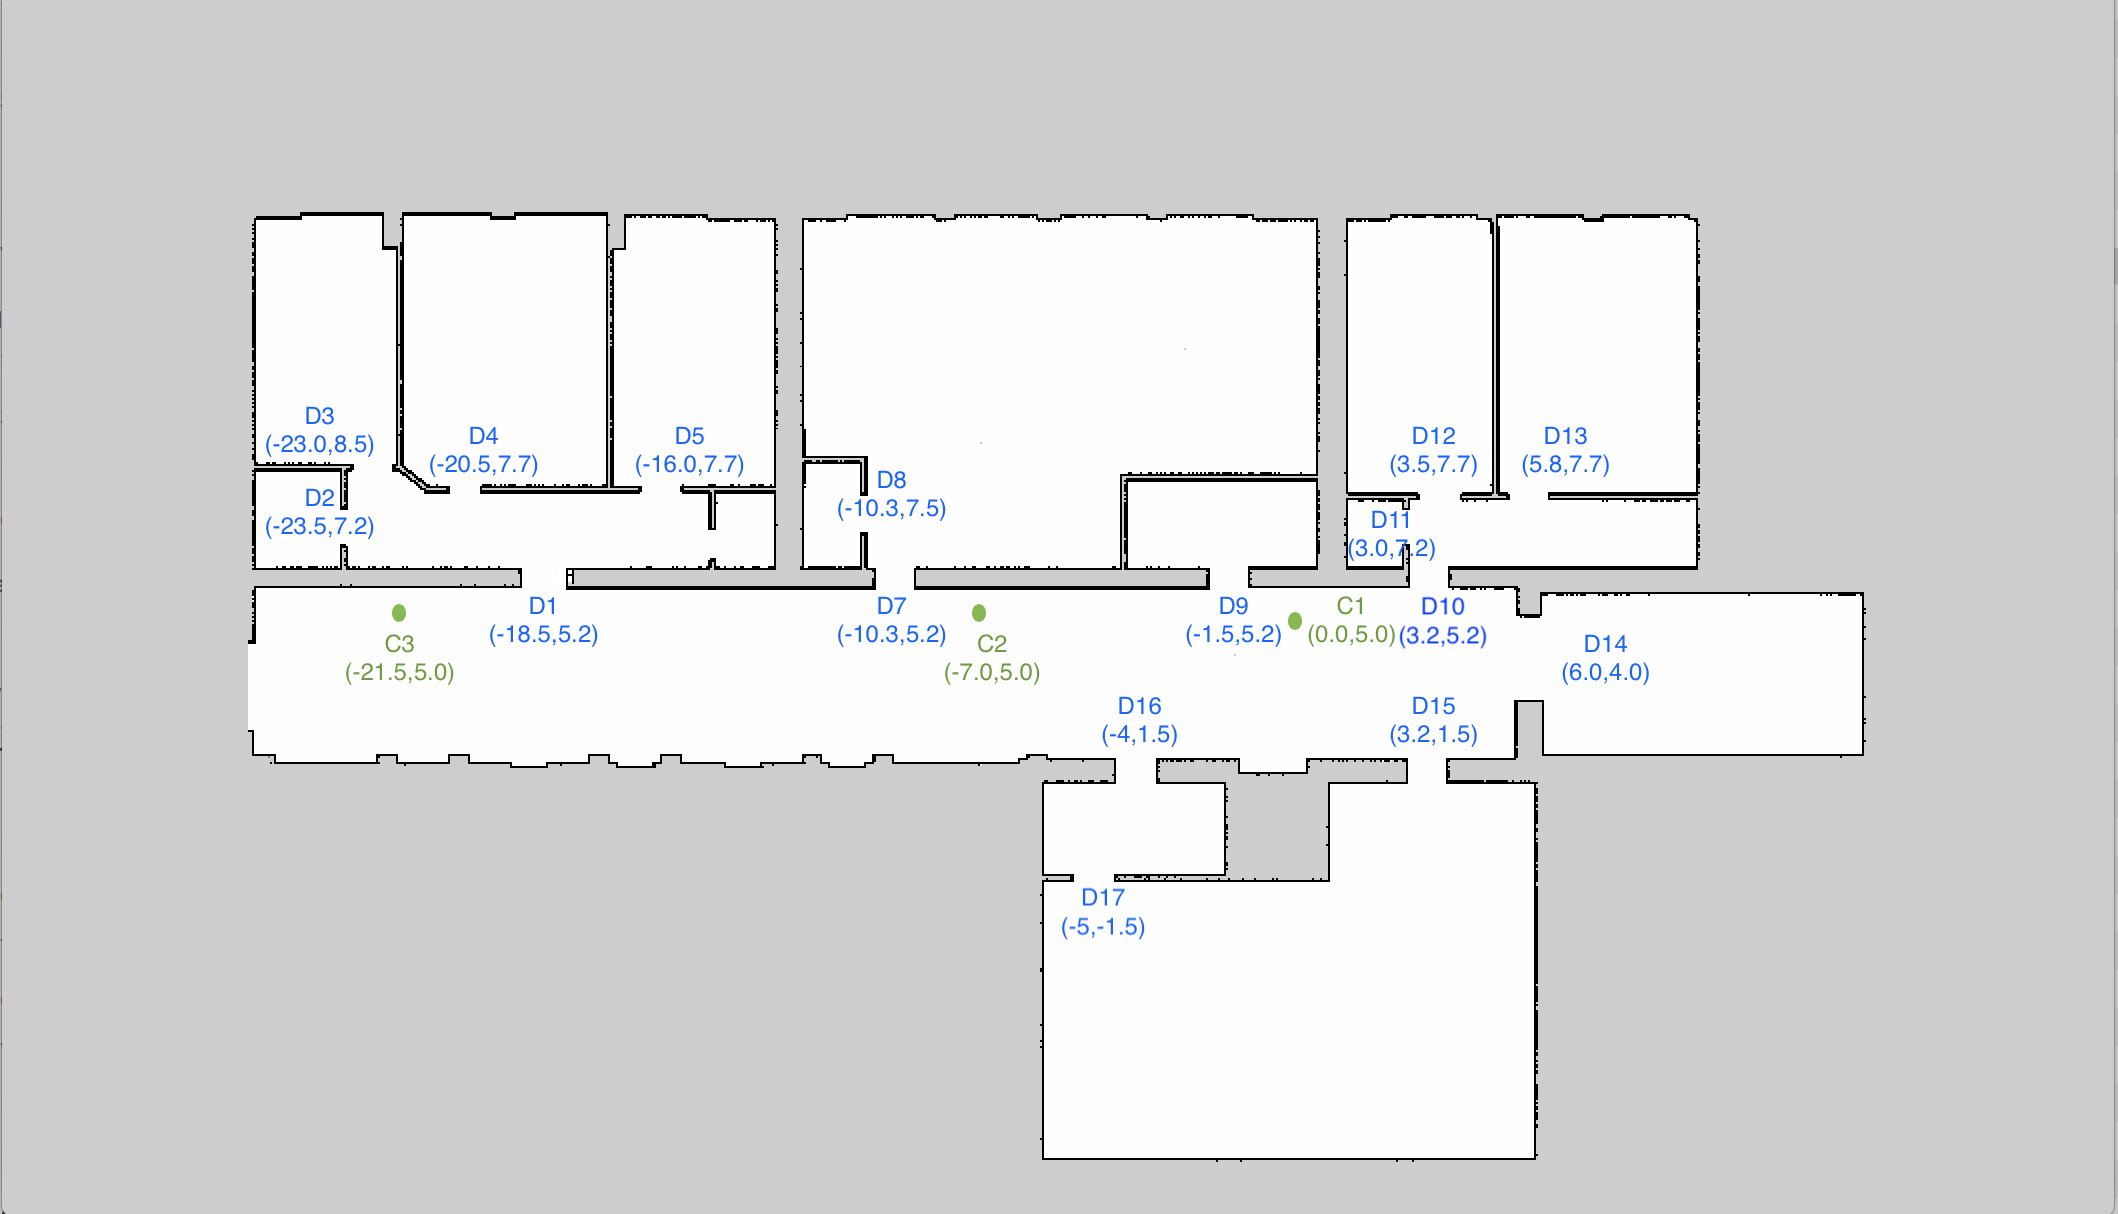
\includegraphics[width = 0.7\textwidth]{content/images/ch3/positions_door_station.png}
	\caption{Doors and Charging Stations}
	\label{fig:positions_door_station}
\end{figure}

\section{Task allocation}

\subsection{Task explanation}
\label{sec:task_explanation}
In order to improving overall execution efficiency. One single robot can carry either small task, which make robot move to one position, or large task, which consist of multiple small task.
On one hand, to make robot work long hours in office enviroment, recharging is necessary. On the other hand, a robot should gather enviroment information as much as possible, which centralized pool would learn from and make better decision. 
Therefore, three types of task are defined, which are shown in Table \ref{fig:task_types}. 

\begin{figure}[htb]
	\centering
	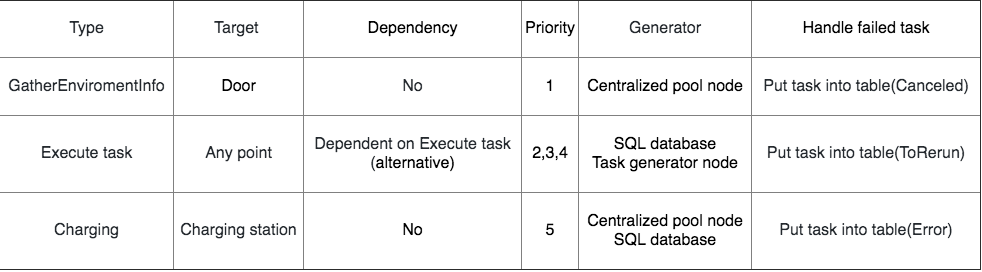
\includegraphics[width = 0.8\textwidth]{content/images/ch3/task_types.drawio.png}
	\caption{Comparision of task types }
	\label{fig:task_types}
\end{figure}

\begin{itemize}
	\item \textsl{Task size.} One single robot is able to carry out one charging task or gather inviroment information task, but can carry multiple execute task, thereby 
	These tasks with dependencies also referred to as small task. Those small tasks form a dependency chain, also referred to as a large task.
	\item \textsl{Priority.}
\end{itemize}

\subsection{Task factor}

\subsection{Enviroment factors}
\begin{itemize}
	\item textsl{Room occupancy.}
\end{itemize}
\subsection{Robot factors}
The decrease amount of robot battery is related to robot trajectory. If a robot get a Large execute task that contains n small task, Equation \ref{eq:battery_consumption} can be used to calculate battery consumption.

\begin{equation}
\begin{aligned}
\label{eq:battery_consumption}
&B: Battery\_Consumption\\
&W: Weight \\
B_{large\_task} & = \sum_{task_0}^{task_n} B_{trajectory} \\
& = \sum_{task_0}^{task_N} \sum_{point_0}^{pont_M} [W_{position} \times position\_variation+W_{angle}  \times angle\_variation]\\
& = \sum_{t = task_0}^{task_N} \sum_{p = point_0}^{point_M} [ W_{position} \times \sqrt{(x_p-x_{p-1} )^2+(y_p-y_{p-1} )^2} \\
&   + W_{angle} \times 2 \times \arccos(w_p)] 
\end{aligned}
\end{equation}

\subsection{Cost function}
	A. Cost function for Execute task that contains n small tasks is shown in Equation \ref{eq:large_task_cost}.
\begin{equation}
	\label{eq:large_task_cost}
	\begin{split}
	Cost_{Large\_execute\_task} = \frac{W_{battery} \times Battery\_consum}{n} + W_{waiting} \times Waiting\_time \\
	+ W_{possibility} \times \prod\limits_{i=1}^n Open\_possibility  + W_{priority} \times priority
	\end{split}
\end{equation}
The robot 

 % + wt_wait \times waiting time + \prod\limits_{i=1}^n open possibility+wt_pri × priority
% wt_btr × battery consumption ÷ N + wt_wait × waiting time+ 
\section{Procedure}
The process of 

